\begin{figure*}[h!]
	\vspace{-.0in}
	\setlength{\tabcolsep}{1pt}
	\begin{center}
		\begin{tabular}{ c  c  | c  c  c c  }
			%\hline
			 \hspace*{-1.0cm}  
             \multirow{4}{*}[-0in]{ \rotatebox[origin=t]{0}{ {\vspace*{1in} 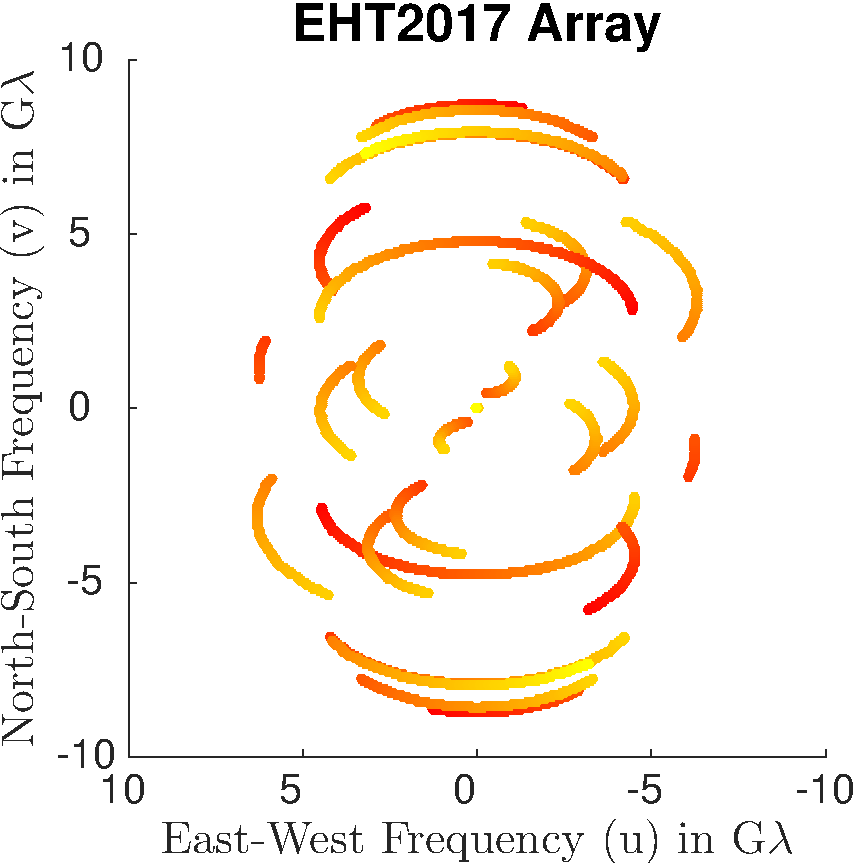
\includegraphics[trim=0cm 0 0 -4cm,height=.43\linewidth]{figures/uvcoverage/uv_eht2017_2.pdf}}
			 		\qquad  }}
			 &  \hspace{-0.7cm}  \large{\textsf{Truth}}   & &  \large{\textsf{a = 2}} & \large{\textsf{a = 5}}  &  \large{\textsf{a = 10}}    \\
			&  \hspace{-0.5cm} {{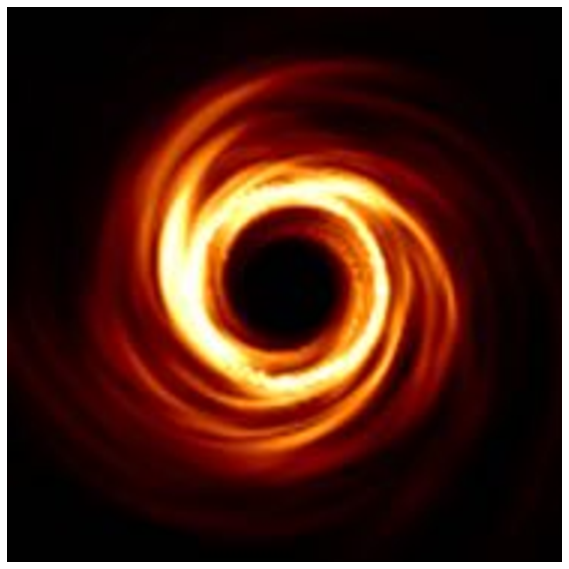
\includegraphics[height=.13\linewidth]{figures/singleimage/visibilities/hotakaframe3.pdf}} } &
			\multirow{1}{*}[0.82in]{ \rotatebox[origin=t]{90}{ \small{\textsf{Gauss. Recon.}} }}
			&
			{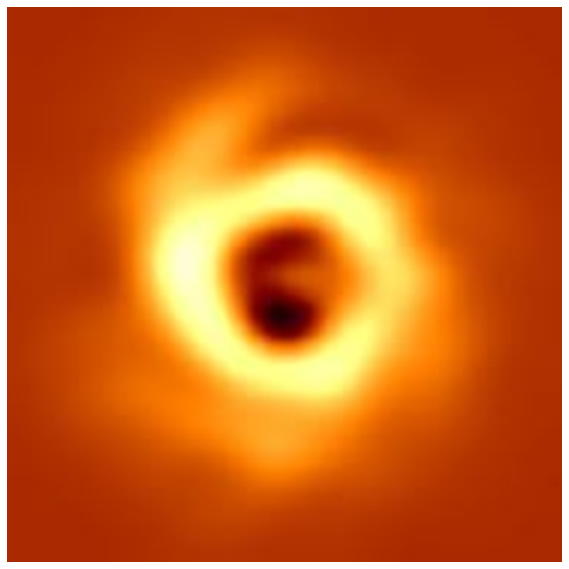
\includegraphics[height=.13\linewidth]{figures/singleimage/visibilities/img_powerdropoff_2.pdf}} &
			{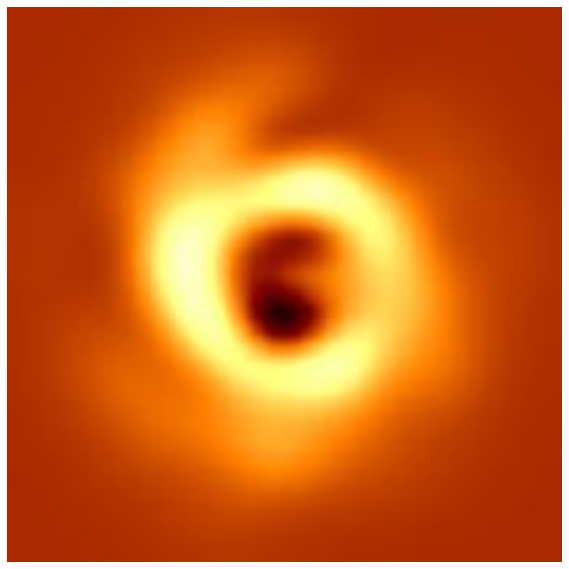
\includegraphics[height=.13\linewidth]{figures/singleimage/visibilities/img_powerdropoff_5.pdf}} 
			&
			{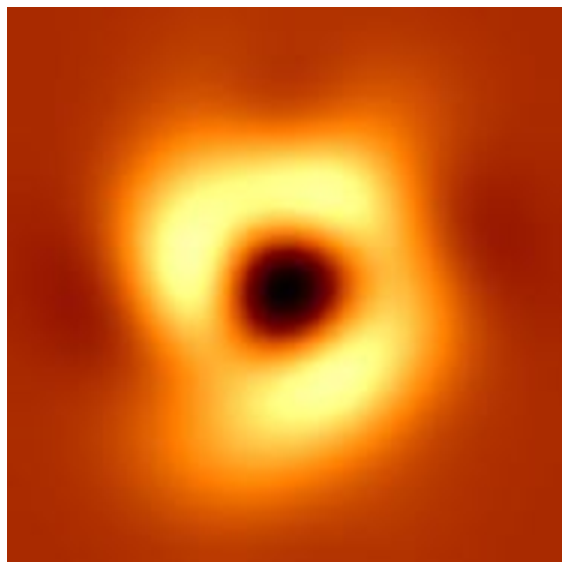
\includegraphics[height=.13\linewidth]{figures/singleimage/visibilities/img_powerdropoff_10.pdf}} 
			\\
			& \vspace{-.0in}  \hspace{-0.8cm} \large{\textsf{MEM \& TV}}  & &  \multicolumn{3}{c}{ 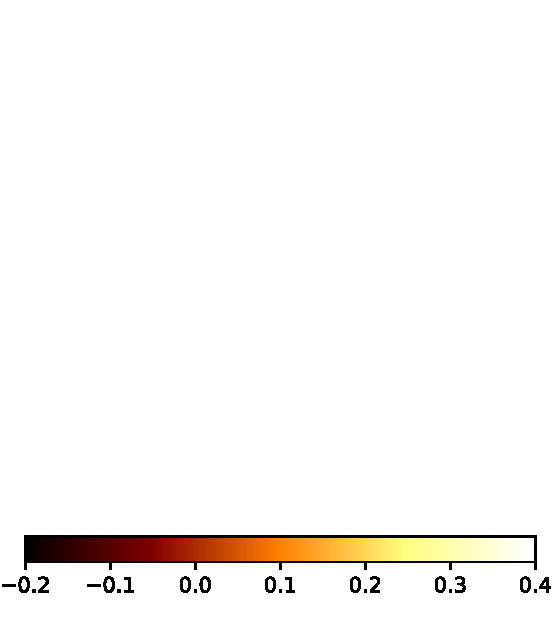
\includegraphics[width=.25\linewidth]{figures/cbar/horizontal_cbar_-2to4_r2.pdf} }
			\\
			%& \vspace{-.15in}  \hspace{-0.8cm} \large{\textsf{MEM \& TV}}  & & & &       \\
			&\hspace{-0.5cm} {{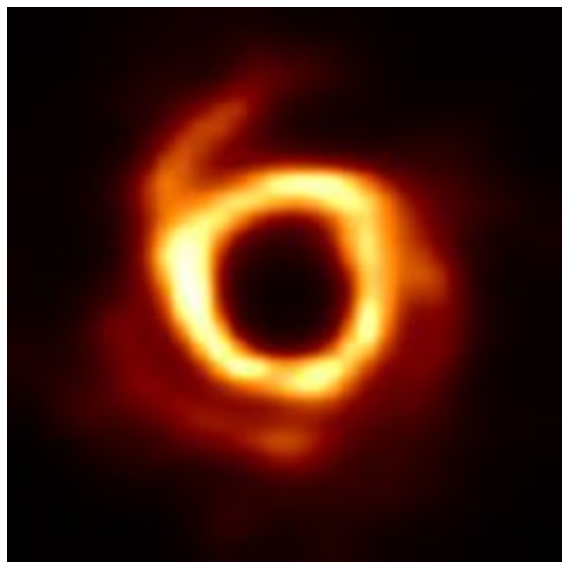
\includegraphics[height=.13\linewidth]{figures/singleimage/visibilities/img_maxen.pdf}} } &
			\multirow{1}{*}[0.82in]{ \rotatebox[origin=t]{90}{ \small{\textsf{Clipped Recon.}} }}
			&
			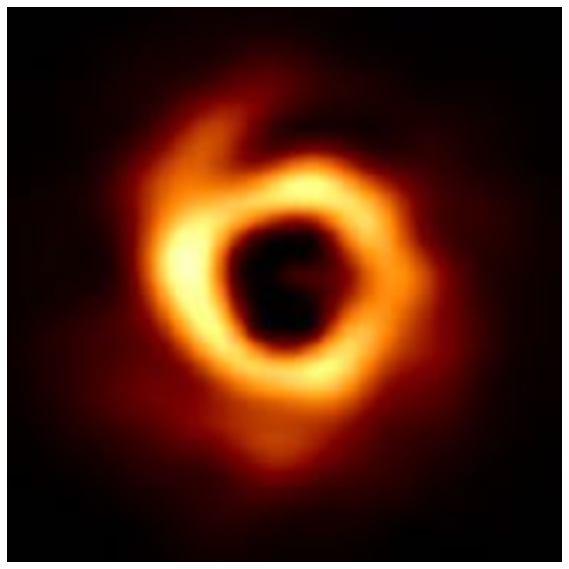
\includegraphics[height=.13\linewidth]{figures/singleimage/visibilities/imgClip_powerdropoff_2.pdf} &
			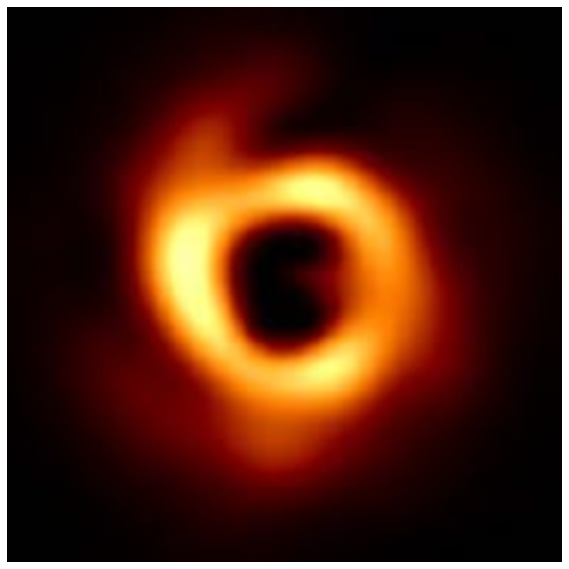
\includegraphics[height=.13\linewidth]{figures/singleimage/visibilities/imgClip_powerdropoff_5.pdf} &
			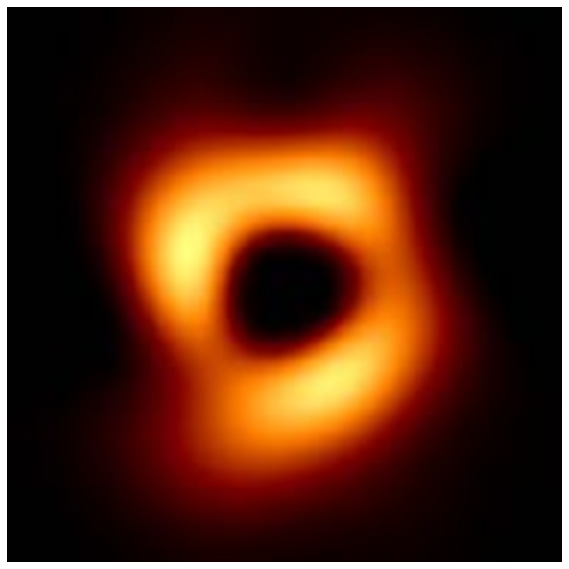
\includegraphics[height=.13\linewidth]{figures/singleimage/visibilities/imgClip_powerdropoff_10.pdf} 
			\\
			& \vspace{-.0in} \hspace{-.8cm} \large{\textsf{CHIRP}}  & &  \multicolumn{3}{c}{ 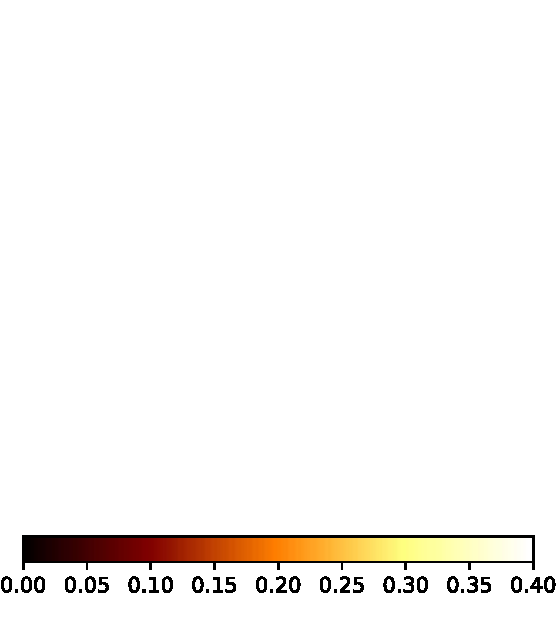
\includegraphics[width=.25\linewidth]{figures/cbar/horizontal_cbar_0to4_r2.pdf} }
			\\ 
			%& \vspace{-.15in} \hspace{-.8cm} \large{\textsf{CHIRP}}   & & & &     \\
			&\hspace{-0.5cm} {{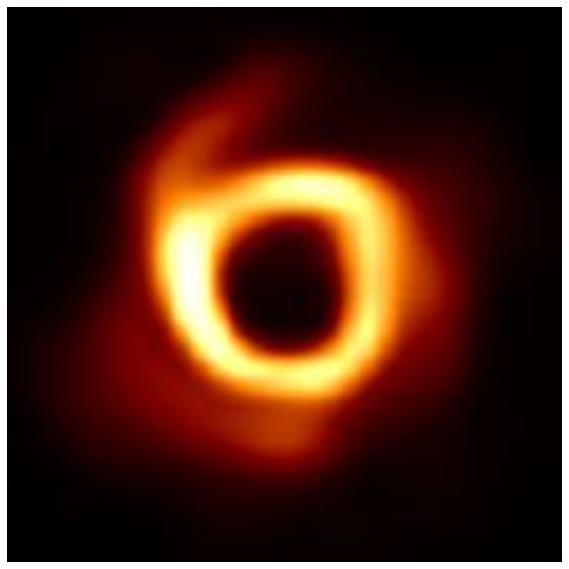
\includegraphics[width=.13\linewidth,trim=0.0cm -1.5cm 0.0cm 0.0cm]{figures/singleimage/visibilities/hotakaframe_chirp.pdf}} \vspace{0.04cm} } &
			\multirow{1}{*}[1.05in]{ \rotatebox[origin=t]{90}{ \small{\textsf{Diagonal Std. Dev. }} }}
			&
			\hspace{-.1in} 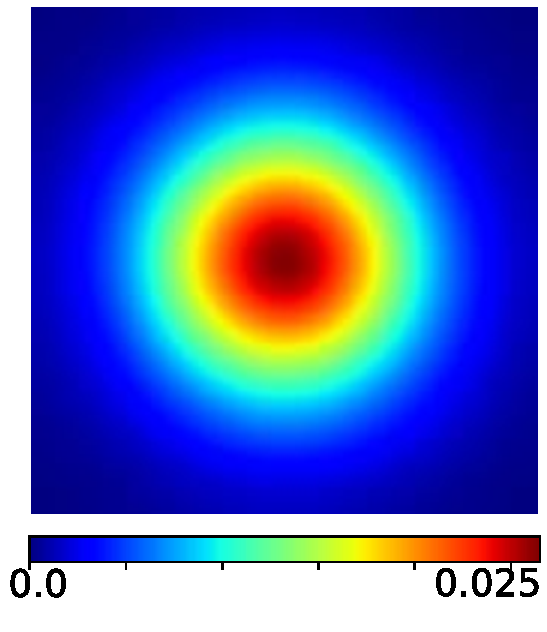
\includegraphics[width=.138\linewidth]{figures/singleimage/visibilities/covImg_powerdropoff_2_r2.pdf} &
			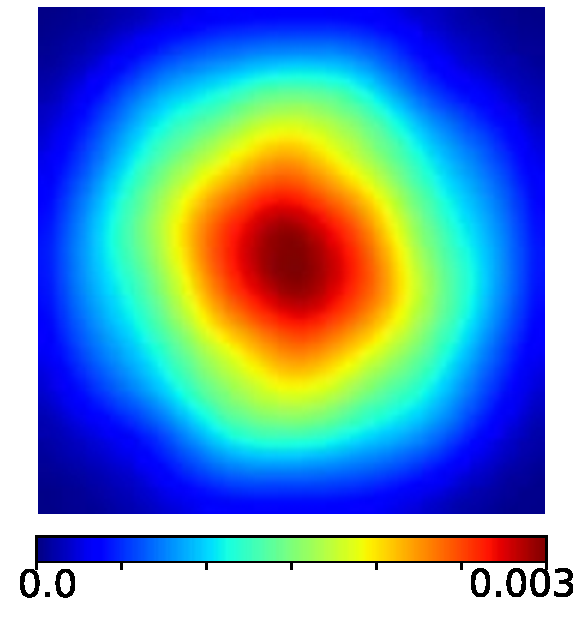
\includegraphics[width=.148\linewidth]{figures/singleimage/visibilities/covImg_powerdropoff_5_r2.pdf} 
			&\hspace{-.1in}
			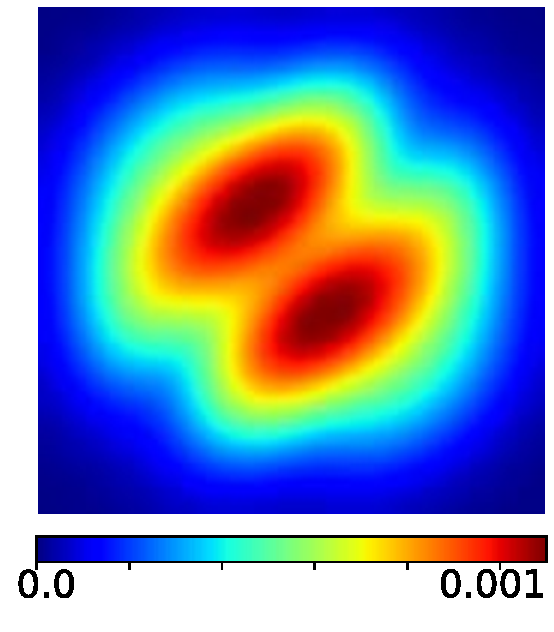
\includegraphics[height=.145\linewidth]{figures/singleimage/visibilities/covImg_powerdropoff_10_r2.pdf} 
		\end{tabular}
		\caption{{\bf Static Imaging Comparison:} Results of static imaging using a multivariate Gaussian prior ( \textsf{a} = 2, 5, 10) compared to state-of-the-art reconstruction methods using MEM \& TV regularizers~\cite{andrew} as well as patch-based regularizers (CHIRP)~\cite{bouman2016computational}. All images are shown with a field of view of 160 $\mu$-arcseconds. Data is generated using a static image with the uv-coverage of the EHT2017 array shown on the left (see Section~\ref{sec:results}). The uv-coverage is colored by time, as indicated by the colorbar in Figure~\ref{fig:uvcov2}. Note however that in this static imaging case the time of measurements is not relevant. Although the previous algorithms (MEM \& TV and CHIRP) both produce better results, the Gaussian reconstruction is able to correctly get the broad structure of the underlying image. Since we do not impose positivity, negative values are reconstructed. However, by clipping the resulting image we can see that the result aligns well with the true static image. The Gaussian prior model also allows us to easily estimate our reconstructed image uncertainty. We visualize the diagonal entries of the posterior covariance matrix as the reshaped standard deviation image. Note that as the smoothness parameter \textsf{a} is increased, the per-pixel standard deviation becomes smaller, but the structure of the standard deviation deviates from what was specified in the prior (recall $\bLambda$ is scaled by $\bmu$, which we have specified as a 2D Gaussian in this work). For large \textsf{a} the uncertainty is shown to be primarily in the diagonal north-west to south-east direction, due to the lack of spatial frequencies sampled by the telescope array in this direction. To avoid approximations and best show the recovered posterior covariance matrices, atmospheric error has not been included in the data used to recover these images. The scaling of the colormaps is in mili-Jansky per squared $\mu$-arcsecond. } 
		\label{fig:staticimaging}
		%-.2, .4
		%0, .4
	\end{center}
	\vspace{-.2in}
\end{figure*}